%
\documentclass[a4paper,12pt]{article}
% Глобальные параметры
\usepackage[T2A]{fontenc}  % кириллический набор символов
\usepackage{cmap} % русские буквы в поиске PDF
\usepackage[utf8]{inputenc}
\usepackage[english, russian]{babel}  % настройки для русской типографики и переносов
\usepackage{fullpage, anysize} %http://texdoc.net/texmf-dist/doc/latex/preprint/fullpage.pdf
%Full page with small margins. 
\usepackage{verbatim}
%Package to display text as in editor.
%\usepackage{minitoc} 
\usepackage{mathtext} 
%maybe without l. Russian letters in math
\usepackage{graphicx}
\usepackage{caption2}
%Some new ways to make caption
\usepackage{amssymb,amsmath} 
%American mathematic styles.
\usepackage{hhline}
%Complex tables making
%texnames - Display TeX.
%subfigure 
\usepackage{multicol, wrapfig}%multi column text and wrap images.
\renewcommand{\captionlabeldelim}{.}%doesn't work in caption package.
% \sloppy
% This declaration makes TeX less fussy about line breaking. This can prevent overfull boxes, but may leave too much space between words.
\raggedbottom
%Makes all pages the height of the text on that page. No extra vertical space is added.

\newcommand{\limp}{\Rightarrow}
\newcommand{\leqs}{=}
\newcommand{\lors}{\|}
\newcommand{\lands}{\&\&}

% Библиография: обычный размер!
\makeatletter
\renewenvironment{thebibliography}[1]{%
  \@xp\section\@xp*\@xp{\bibname}%
  \normalfont\labelsep .5em\relax
  \renewcommand\theenumiv{\arabic{enumiv}}\let\p@enumiv\@empty
  \list{\@biblabel{\theenumiv}}{\settowidth\labelwidth{\@biblabel{#1}}%
    \leftmargin\labelwidth \advance\leftmargin\labelsep
    \usecounter{enumiv}}%
  \sloppy \clubpenalty\@M \widowpenalty\clubpenalty
  \sfcode`\.=\@m
}
\makeatother

\endinput

%\begin{thebibliography}{2005}
%
%\bibitem{texbook} D.~E.~Knuth. UML: Основы. 2002. Перевод с английского: СПБ. ~--- 192с.
%
%
%\bibitem{manual} B Cloves Carneiro Jr., and Rida Al Barazi. Beginning Rails 3. 2010. ~--- 403c.
%
%\bibitem{roganov}
%Е.А. Роганов
%{\em Название книги.}~---
%М., Издательство, 2001.
%Что-либо ещё.
%
%\end{thebibliography}
%
%\endinput

\title{Поиск ассоциативных правил оценки количества лесных пожаров в модели ANFIS.}
\author{Костенчук М.И.}

\date{01-03-2014}

\begin{document}

\maketitle

\section{Введение}

% Прогноз пожароопасной обстановки: http://www.rosleshoz.gov.ru/forest_fires/prediction
% http://www.rosleshoz.gov.ru/forest_fires/prediction класс природной пожарной опасности в лесах в зависимости от условий погоды
%Тема доклада: Построение ассоциативных правил, выражающих зависимость количества лесных пожаров от погодных условий.
%Цель: Снижение рисков и смягчение последствий лесных пожаров.
%Задача: Разработка специализированного программного обеспечения для нахождения ассоциативных правил, выражающих зависимость количества лесных пожаров от погодных условий в среде разработки Qt.
%Объект: Динамика возникновения лесных пожаров.
%Предмет: Зависимость возникновения лесных пожаров от погодных условий.
%Метод: Математическое моделирование основанное на нечёткой логике.

Россия по праву считается лесной державой, на неё приходится 1/5 часть всех лесов мира, 1/2 часть всех хвойных лесов, леса занимают ~50\% всей площади страны и составляют 1,2 млрд. га.
 
На территории лесного фонда России ежегодно регистрируется от 10 до 35 тыс. лесных пожаров, охватывающих площади от 0,5 до 2,5 млн. га. С учетом горимости огромного количества лесов на неохраняемых и эпизодически охраняемых территориях северных районов Сибири и Дальнего Востока общая величина пройденной огнем площади составляет от 2,0 до 5,5 млн. га.
 
При этом ущерб от лесных пожаров в 2013 году составил порядка 20 млрд рублей.

%
%
%Ущерб от лесных пожаров в 2013 году на территории России составил 20 миллионов рублей
%в 2013 году площадь лесных пожаров в России уменьшилась по сравнению с прошлым годом и составила 1,4 миллиона гектаров.
%
%
%%РИА Новости http://ria.ru/eco_news/20131213/983924582.html#ixzz2usMksJpD
%
%ущерб от лесных пожаров в 2013 году составил порядка 20 млрд рублей
%
%%Подробности: http://www.regnum.ru/news/1745253.html#ixzz2usNpw0dp 
%
%
%Данные сайта МЧС Прямой материальный ущерб от пожаров, тыс. руб. (в целых) 8367611
%
%% http://www.gks.ru/free_doc/new_site/business/sx/les2.htm

%%%%%%%%%%%%%%%%%%%%%%%%%%%%%%%%%%%%
\section{Постановка задачи}
Точный прогноз количества пожаров в регионе позволяет снизить количество пожаров, а также ущерб, наносимый в результате их возникновения. Отсюда вытекает цель данной работы~--- снизить риски и смягчить последствия лесных пожаров. Объектом исследования является динамика возникновения лесных пожаров в рассматриваемом регионе. Предметом~--- зависимость возникновения лесных пожаров от погодных условий. Для достижения цели, поставлена задача разработки специализированного программного обеспечения для нахождения ассоциативных правил выражения зависимости количества лесных пожаров от погодных условий в среде разработки Qt. Методом, с помощью которого производится разработка, является математическое моделирование, основанное на нечёткой логике.

Очевидно, что горимость лесов в большой степени зависит от температуры и сухости воздуха (дефицита влажности): чем выше температура и сухость воздуха, тем больше горимость и наоборот. Так же очевидно и то, что на пожароопасную обстановку влияет скорость ветра и количество осадков.

Для выявления этого влияния используется модель Нейронной Нечёткой Продукционной Сети(ННПС) ANFIS, реализующая алгоритм нечёткого вывода Цукамото.

ННПС ANFIS это 5-слойная нейронная сеть, которой на вход поступают численные значения параметров, а на выходе получается результат нечёткого вывода (Рис. \ref{anfis_png}). 


\begin{center}
  \makebox[\textwidth]{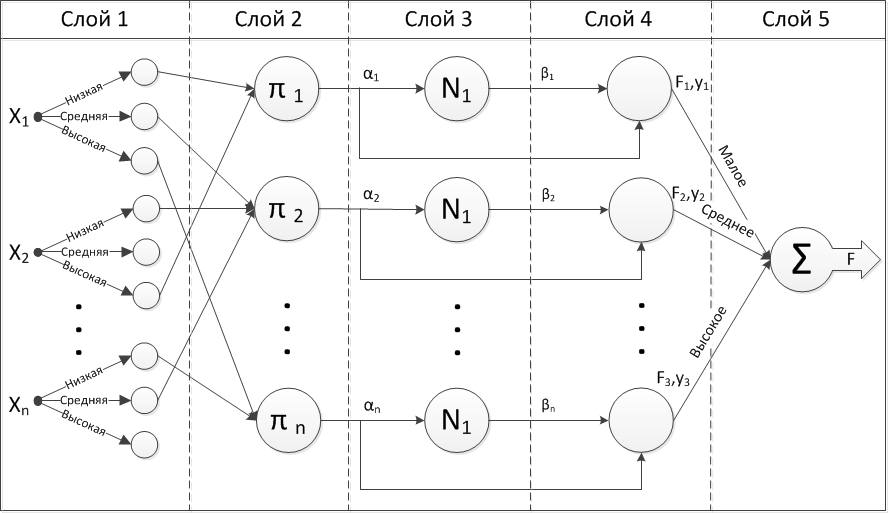
\includegraphics[width=\textwidth]{anfis.png}}
  \captionof{figure}{\label{anfis_png} Нейронная нечёткая продукционная сеть ANFIS}
\end{center}

Подробное рассмотрение сети выходит за рамки исследования. Данная работа посвящена построению второго слоя ННПС, который представляет из себя набор правил нечёткого вывода. 

Правилом нечёткого логического вывода называется правило получения заключения в виде нечёткого множества, соответствующего текущим значениях входов, с использованием нечеткой базы знаний и нечетких операций и отражающее наиболее распространённые закономерности, связывающие предпосылку и результат.

Для нахождения этих зависимостей будем использовать алгоритм интеллектуального анализа данных Apriori. Данный алгоритм позволяет за время существенно меньшее, чем полный перебор найти в базе данных наиболее часто встречающиеся наборы.

\section{Алгоритм Apriori}

Алгоритм построен на основе принципа антимонотонности, который гласит, что поддержка набора (т.е. частота, с которой он встречается в базе данных) с увеличением числа элементов в нём уменьшается или остаётся прежней. Исходя из этого на первом шаге алгоритма вычисляется поддержка всех наборов с максимальной поддержкой, т.е. наборов единичной длины. И для каждого из элементов, поддержка которого превышает минимальный порог создаётся вершина дерева. Дальше к каждой вершине рекурсивным образом добавляются все элементы того же уровня лежащие правее и поддержка набора, составленного из пути от вершины и нового элемента которых, выше установленного порога. Таким образом получается дерево наиболее частых наборов(Рис. \ref{apriori_tree_png}), которые можно получить, используя обход дерева в глубину. Пути от каждого элемента до корня дерева являются искомыми наборами.

\begin{center}
  \makebox[\textwidth]{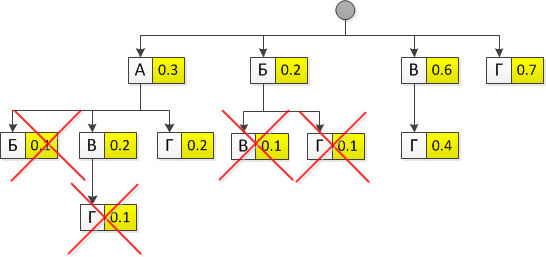
\includegraphics[width=\textwidth]{Apriori_Tree.png}}
  \captionof{figure}{\label{apriori_tree_png} Дерево частых наборов}
\end{center}




%\begin{figure}[h]
%    \centering
%    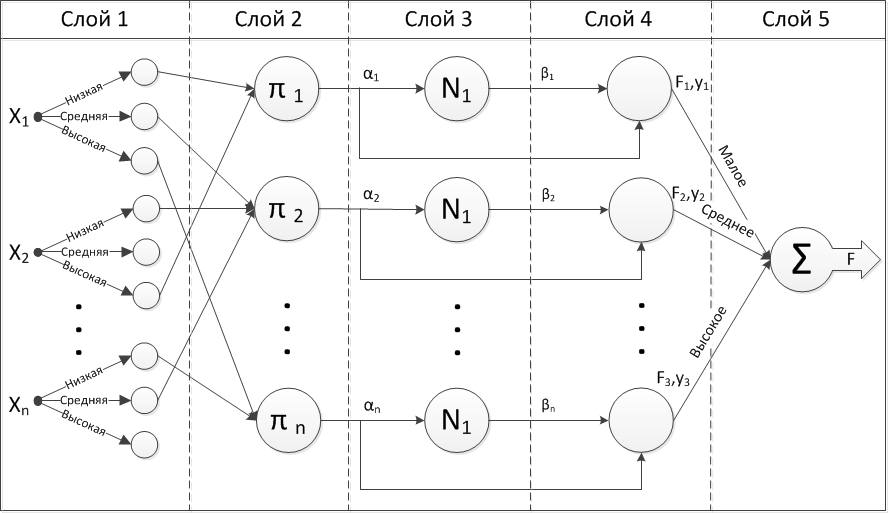
\includegraphics[width=1.0\textwidth]{anfis.png} 
%    \hfill\hfill
%    \caption{Нейронная нечёткая продукционная сеть ANFIS} 
%    \label{anfis_png} 
%\end{figure}








\begin{enumerate}
\end{enumerate}

?

Здесь будет немного текста. 
\(f= 1/2\frac{a\sqrt{i}}{b}\)





\end{document}
